\subsection[]{Grundlagen}

\begin{frame}{Szintillatoren}

\begin{description}
	  \item[Szintillatoren] bestehen aus Material, dessen Moleküle nach Anregung durch geladene
	  Teilchen oder Photonen die Anregungsenergie in Form von Licht wieder abgeben
	\end{description}
	\begin{block}{Arten}
		\begin{itemize}
		  \item organische Szintillatoren (Kristalle, Gläser, Edelgase)
		  \item anorganische Szintillatoren (Kristalle, Flüssigkeiten, Plastik)
		\end{itemize}
	\end{block}
	\begin{block}{Organische Szintillatoren}
		\begin{itemize}
		  \item aromatische Kohlenwasserstoffverbindungen
		  \item hauptsächlich organische Kristalle oder Plastikszintillatoren
		  \item Wechsel eines freien Valenzelektrons zw.
Molekülorbitalen verschiedener Energie unter Abgabe eines Photons
		  \item Bsp.: C$_{10}$H$_8$, C$_{14}$H$_{10}$
		\end{itemize}
	\end{block}
\end{frame}	


% \begin{frame}{Szintillatoren}
% % 	\begin{block}{Anorganische Szintillatoren}
% % 		\begin{itemize}
% % 		  \item anorganische Kristalle mit eingebrachten Fremdatomen (Aktivatorzentren) $\rightarrow$
% % 		  zusätzliche Energieniveaus
% % 		  \item durch eintreffende Strahlung angeregtes $e^-$ wandert durch Kristall, bis es auf Loch
% % 		  trifft und rekombiniert $\rightarrow$ Abgabe eines Photons
% % 		  \item Bsp.: NaI,CsI, BaF$_2$,
% % 		\end{itemize}
% % 	\end{block}
% % 		\begin{block}{Organische Szintillatoren}
% % 		\begin{itemize}
% % 		  \item aromatische Kohlenwasserstoffverbindungen
% % 		  \item hauptsächlich organische Kristalle oder Plastikszintillatoren
% % 		  \item Wechsel eines freien Valenzelektrons zw.
% % Molekülorbitalen verschiedener Energie unter Abgabe eines Photons
% % 		  \item Bsp.: C$_{10}$H$_8$, C$_{14}$H$_{10}$
% % 		\end{itemize}
% % 	\end{block}
% \end{frame}	

	
\subsection[]{Szintillationszähler}



\begin{frame}{Szintillationszähler}
	\begin{columns}[T]
		\column{.65\textwidth}
			\begin{itemize}
			  \item Bündelung von Szintillationsfasern ($\varnothing~<$~1~mm) $\rightarrow$
			  Ineffizienzenausgleich
			  \item parallele Bündel ergeben eindimensionale Ortsinformation
			  \item in Winkel aufeinander stehende Ebenen ergeben zwei- bzw. dreidimensionale Ortsinformation
			  \item oft 1-2 Mäntel um Fasern, um Lichtausbeute zu erhöhen
			  \item Anordnung der Faser je nach Detektorgeometrie
			  \item Auslese durch Photomultiplier
			\end{itemize}	
	    \column{.4\textwidth}
	    	\begin{figure}[htbp]
			  \centering
			  \includesvg[svgpath=bilder/, width=\columnwidth]{szintillator-fasern}
% 			  \caption{Aufbau eines Szintillationszählers}
			\end{figure}
    \end{columns}
\end{frame}	

\begin{frame}{Szintillationszähler}
		\begin{columns}[T]
		\column{.65\textwidth}
			\begin{figure}[htbp]
			  \centering
			  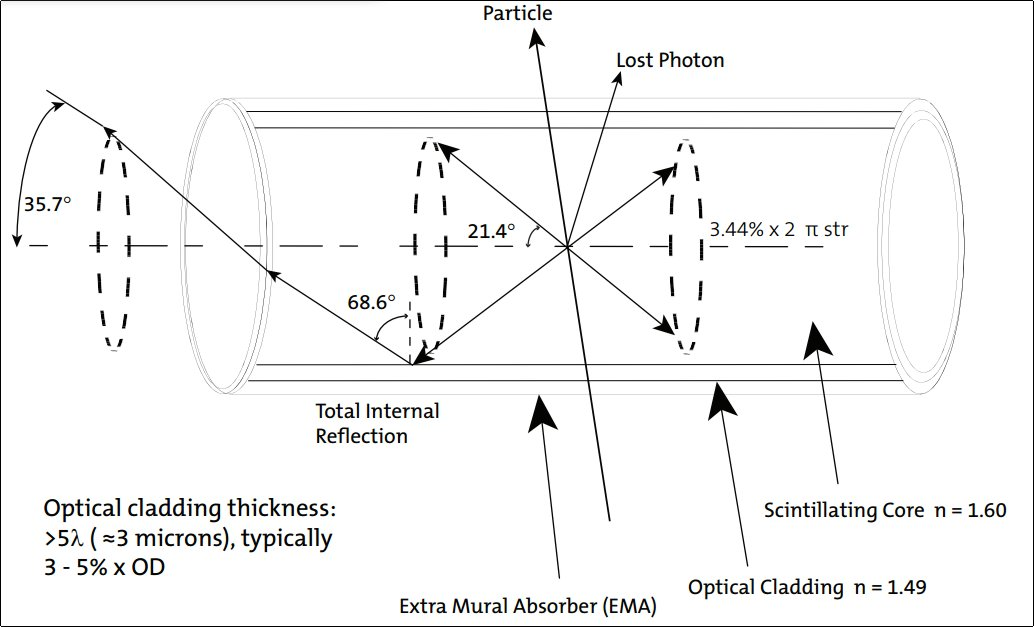
\includegraphics[width=\textwidth]{szintifibre.jpg}
			  \caption*{[stg]}
			\end{figure}
	    \column{.4\textwidth}
	    	\begin{figure}[htbp]
			  \centering
			  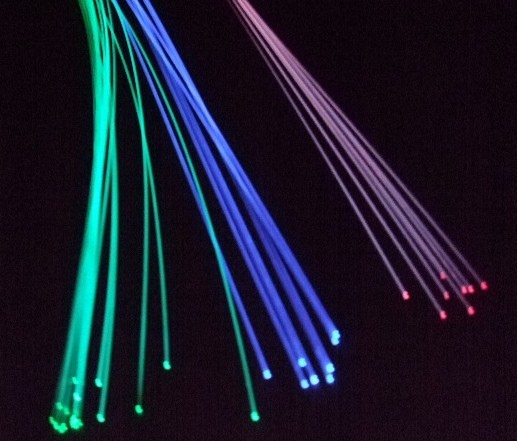
\includegraphics[width=\textwidth]{szintifasern.jpg}
			  \caption*{[scf]}
			\end{figure}
    \end{columns}
\end{frame}
	
	\begin{frame}{Szintillationszähler}
    \begin{columns}[T]
		\column{.45\textwidth}
			\textbf{Vorteile}		
			\vspace{0.7cm}
			\begin{itemize}
			  \item an Geometrie anpassbar (krümmbar)
			  \item wenig Masse (wenig Vielfachstreuung)
			  \item geringe Antwortzeit (10-15~ns)
			  \item gute Ortsauflösung ($O(100\mu m)$)
			  \item wenig Infrastruktur (Gaszuleitungen etc)
			\end{itemize}	
	    \column{.5\textwidth}
	    	\textbf{Nachteile}
	    	\vspace{0.7cm}
	    	\begin{itemize}
			  \item geringe Lichtausbeute (ca. 5\%)
			  \item Lichtausbeute stark von Oberflächengüte abhängig (Schmutz, Kratzer)
			\end{itemize}
    \end{columns}
\end{frame}

\begin{frame}{Szintillationszähler}
% 		\begin{columns}[T]
% 		\column{.65\textwidth}
% 			\begin{figure}[htbp]
% 			  \centering
% 			  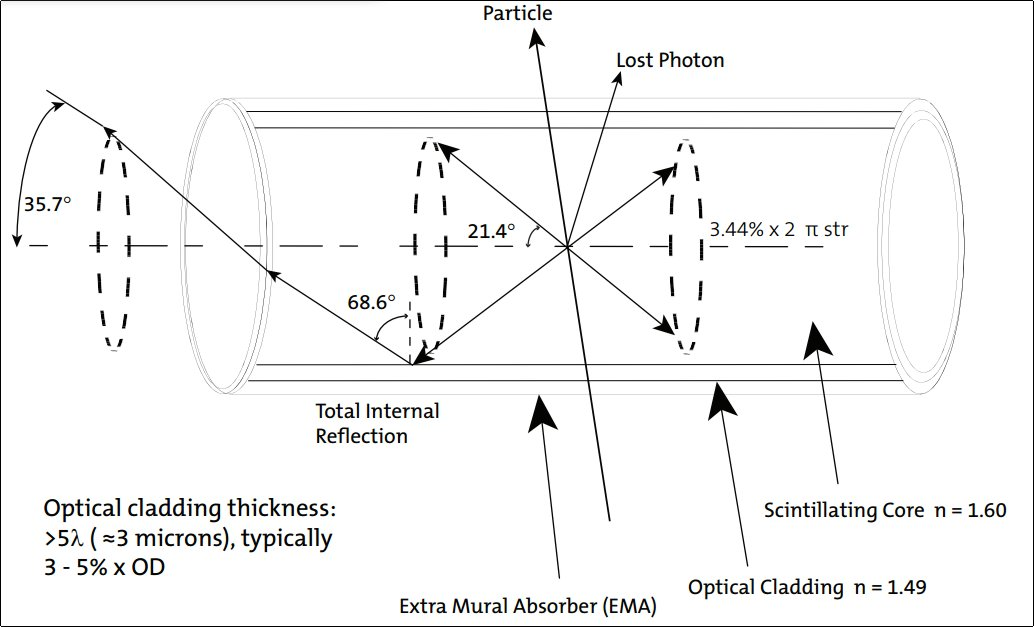
\includegraphics[width=\textwidth]{szintifibre.jpg}
% 			\end{figure}
% 	    \column{.4\textwidth}
% 	    	\begin{figure}[htbp]
% 			  \centering
% 			  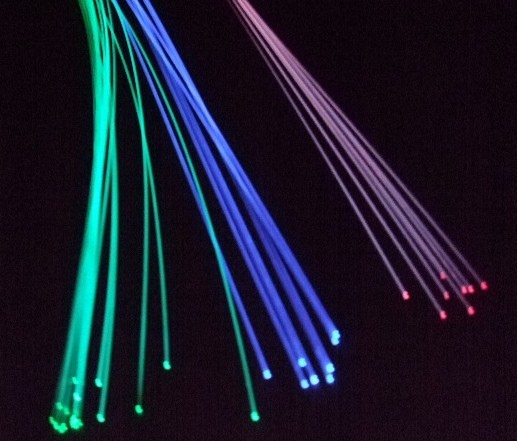
\includegraphics[width=\textwidth]{szintifasern.jpg}
% 			\end{figure}
%     \end{columns}
Beispielbild
\end{frame}
